%%%%%%%%%%%%%%%%%%%%%%%%%%%%%%%%%%%%%%%%%%%%%%%%%%%%%%%%%%%%%%%%%%%%%%%%%%%%%%%%
% Template for USENIX papers.
%
% History:
%
% - TEMPLATE for Usenix papers, specifically to meet requirements of
%   USENIX '05. originally a template for producing IEEE-format
%   articles using LaTeX. written by Matthew Ward, CS Department,
%   Worcester Polytechnic Institute. adapted by David Beazley for his
%   excellent SWIG paper in Proceedings, Tcl 96. turned into a
%   smartass generic template by De Clarke, with thanks to both the
%   above pioneers. Use at your own risk. Complaints to /dev/null.
%   Make it two column with no page numbering, default is 10 point.
%
% - Munged by Fred Douglis <douglis@research.att.com> 10/97 to
%   separate the .sty file from the LaTeX source template, so that
%   people can more easily include the .sty file into an existing
%   document. Also changed to more closely follow the style guidelines
%   as represented by the Word sample file.
%
% - Note that since 2010, USENIX does not require endnotes. If you
%   want foot of page notes, don't include the endnotes package in the
%   usepackage command, below.
% - This version uses the latex2e styles, not the very ancient 2.09
%   stuff.
%
% - Updated July 2018: Text block size changed from 6.5" to 7"
%
% - Updated Dec 2018 for ATC'19:
%
%   * Revised text to pass HotCRP's auto-formatting check, with
%     hotcrp.settings.submission_form.body_font_size=10pt, and
%     hotcrp.settings.submission_form.line_height=12pt
%
%   * Switched from \endnote-s to \footnote-s to match Usenix's policy.
%
%   * \section* => \begin{abstract} ... \end{abstract}
%
%   * Make template self-contained in terms of bibtex entires, to allow
%     this file to be compiled. (And changing refs style to 'plain'.)
%
%   * Make template self-contained in terms of figures, to
%     allow this file to be compiled. 
%
%   * Added packages for hyperref, embedding fonts, and improving
%     appearance.
%   
%   * Removed outdated text.
%
%%%%%%%%%%%%%%%%%%%%%%%%%%%%%%%%%%%%%%%%%%%%%%%%%%%%%%%%%%%%%%%%%%%%%%%%%%%%%%%%

\documentclass[letterpaper,twocolumn,10pt]{article}
\usepackage{usenix-2020-09}

% to be able to draw some self-contained figs
\usepackage{tikz}
\usepackage{amsmath}
\usepackage{graphicx}
\usepackage{xurl} % better URL line breaking

% Import bib file
\addbibresource{citations.bib}

% Improve line breaking to reduce Underfull \hbox warnings in two-column layout
\pretolerance=1000
\emergencystretch=3em
\hyphenpenalty=100
\exhyphenpenalty=50

%-------------------------------------------------------------------------------
% Allow line breaks in links
\hypersetup{breaklinks=true}

\begin{document}
\sloppy
\hyphenation{vul-ner-a-bil-i-ty de-tec-tion ju-li-et con-trol-flow rep-re-sen-ta-tion hy-per-pa-ram-e-ter}
%-------------------------------------------------------------------------------

%don't want date printed
\date{}

% make title bold and 14 pt font (Latex default is non-bold, 16 pt)
\title{\Large \bf Graph Neural Networks for Vulnerability Prediction}

%for single author (just remove % characters)
\author{
{\rm Simon Yu}\\
Simon Fraser University
% copy the following lines to add more authors
% \and
% {\rm Name}\\
%Name Institution
} % end author

\maketitle

%-------------------------------------------------------------------------------
\begin{abstract}
%-------------------------------------------------------------------------------
This report presents the implementation and evaluation of a Graph Neural Network (GNN) approach for vulnerability prediction in C/C++ source code. The project successfully developed a complete pipeline from graph extraction using Clang LibTooling to GNN training with PyTorch Geometric. We extracted Abstract Syntax Trees (ASTs) and Control Flow Graphs (CFGs) from 48,105 functions in the Juliet Test Suite, created a hybrid GCN-GAT model architecture, and achieved 81.8\% accuracy in binary vulnerability classification. Our approach demonstrates the feasibility of using graph-based representations for automated vulnerability detection, though challenges remain in handling class imbalance and generalizing beyond synthetic datasets.
\end{abstract}


%-------------------------------------------------------------------------------
\section{Introduction}
%-------------------------------------------------------------------------------

Software vulnerabilities in C/C++ applications pose significant security risks, with manual code review being time-consuming and error-prone for large codebases. This project investigated whether Graph Neural Networks (GNNs) operating on program dependency graphs could effectively predict security "hotspots" in source code functions.

The motivation stems from the need for automated tools that can identify high-risk functions in codebases containing millions of lines of code. Traditional static analysis tools often produce high false positive rates, while machine learning approaches typically rely on superficial code features. Our hypothesis was that leveraging the structural information in program graphs through GNNs could provide more accurate vulnerability detection.

We implemented a complete pipeline using the Juliet Test Suite for C/C++, extracting both Abstract Syntax Trees (ASTs) and Control Flow Graphs (CFGs) from functions using Clang LibTooling, and training a hybrid GCN-GAT model to perform binary classification of vulnerable versus non-vulnerable functions.

%-------------------------------------------------------------------------------
\section{Related Work and Background}
%-------------------------------------------------------------------------------

Several recent works have explored graph-based approaches for vulnerability detection. Devign \cite{devign} demonstrated that GNNs can learn comprehensive program semantics from merged AST and call graphs, achieving state-of-the-art results on vulnerability detection. GraphFVD \cite{graphfvd} focused on property graph-based fine-grained vulnerability detection, while VulChecker \cite{vulchecker} employed graph-based localization techniques. TACSan \cite{tacsan} enhanced traditional vulnerability detection with GNNs, showing improvements over conventional static analysis tools.

%-------------------------------------------------------------------------------
\section{Methodology}
%-------------------------------------------------------------------------------

\subsection{Data Collection and Processing}

We utilized the NIST Juliet Test Suite for C/C++, a comprehensive collection of test cases covering various Common Weakness Enumerations (CWEs). The dataset provides both vulnerable ("bad") and non-vulnerable ("good") function implementations, making it ideal for supervised learning.

Our data processing pipeline consisted of three main stages:

\textbf{Graph Extraction:} We developed a Clang LibTooling-based parser that extracts both ASTs and CFGs from C/C++ functions. The tool processes each function individually, building a vocabulary of AST node types and CFG statement types. Functions containing the substring "bad" in their names are labeled as vulnerable (label 1), while others are labeled as non-vulnerable (label 0).

\textbf{Graph Serialization:} Each function is serialized to JSON format containing: (1) the complete AST structure with node types and hierarchical relationships, (2) CFG blocks with statement sequences and control dependencies, and (3) binary vulnerability labels. This resulted in 48,105 processed functions.

\textbf{Data Transformation:} Using PyTorch Geometric, we convert the JSON representations into graph data objects. AST nodes and CFG statements are mapped to integer indices based on a learned vocabulary. Edge relationships preserve both AST parent-child connections and CFG control flow transitions.

\subsection{Model Architecture}

We implemented a hybrid GCN-GAT model that alternates between Graph Convolutional Network (GCN) and Graph Attention Network (GAT) layers:

\begin{itemize}
\item \textbf{Input Layer:} Embedding layer mapping node type indices to 384-dimensional vectors
\item \textbf{Graph Layers:} 5 alternating GCN/GAT layers with batch normalization and residual connections
\item \textbf{Pooling:} Combined global mean and max pooling for graph-level representations  
\item \textbf{Classification Head:} Multi-layer perceptron with dropout for binary classification
\end{itemize}

The architecture addresses common GNN challenges: batch normalization prevents oversmoothing, residual connections preserve early-layer information, and attention mechanisms in GAT layers focus on relevant code patterns.

\subsection{Training Configuration}

The model was trained with the following configuration:
\begin{itemize}
\item Learning rate: 0.0003 with Reduce\-LROn\-Plateau scheduling
\item Batch size: 32
\item Weight decay: 3e-4 for regularization
\item Early stopping with patience of 15 epochs
\item Data splits: 70\% training, 15\% validation, 15\% testing
\end{itemize}

%-------------------------------------------------------------------------------
\section{Results and Evaluation}
\label{sec:results}
%-------------------------------------------------------------------------------

\subsection{Training Performance}

Our model was trained for 100 epochs with early stopping. Training converged after approximately 50 epochs, achieving the following final metrics:

\begin{itemize}
\item \textbf{Test Accuracy:} 81.8\%
\item \textbf{Precision:} 83.6\% 
\item \textbf{Recall:} 81.8\%
\item \textbf{F1-Score:} 81.3\%
\end{itemize}

The confusion matrix revealed:
\begin{itemize}
\item True Negatives: 8,524 (correctly identified non-vulnerable functions)
\item True Positives: 5,040 (correctly identified vulnerable functions)  
\item False Positives: 465 (non-vulnerable functions misclassified as vulnerable)
\item False Negatives: 2,553 (vulnerable functions missed by the model)
\end{itemize}

\begin{figure}[t]
	\centering
	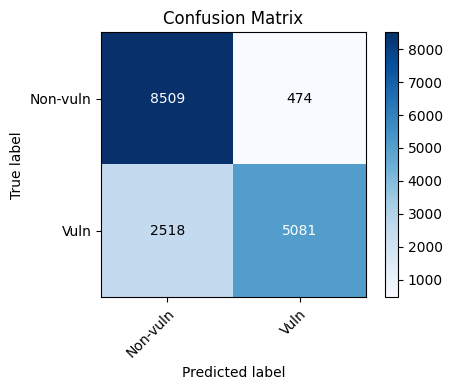
\includegraphics[width=\linewidth]{../model/logs/confusion_matrix.png}
	\caption{Confusion matrix on the test set.}
	\label{fig:confusion-matrix}
\end{figure}

\subsection{Training Dynamics}

The training process showed steady convergence with both training and validation accuracy reaching approximately 82\% by epoch 50. Training loss decreased from 0.64 to 0.40, while validation loss stabilized around 0.41, indicating good generalization without significant overfitting.

The learning rate scheduler activated multiple times during training, reducing the learning rate when validation performance plateaued, which helped achieve final convergence.

\begin{figure}[t]
	\centering
	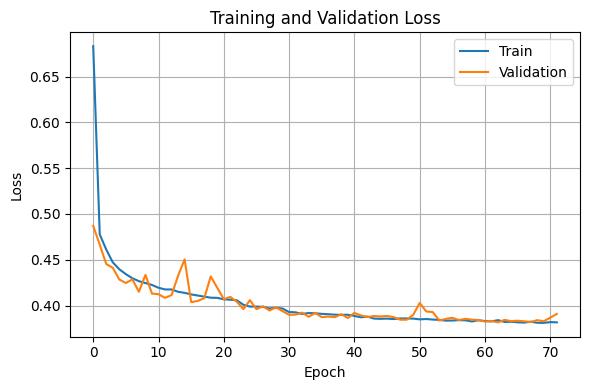
\includegraphics[width=\linewidth]{../model/logs/training_loss.png}
	\caption{Training and validation loss across epochs.}
	\label{fig:training-loss}
\end{figure}

\begin{figure}[t]
	\centering
	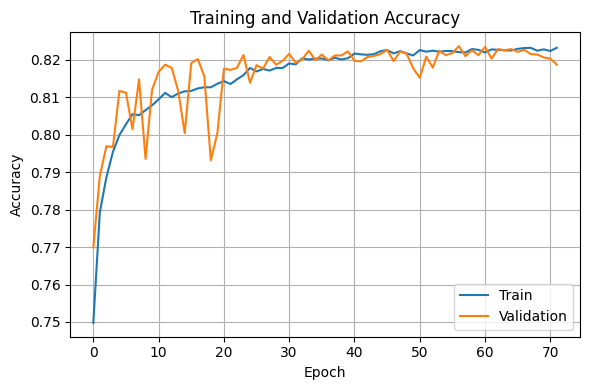
\includegraphics[width=\linewidth]{../model/logs/training_accuracy.png}
	\caption{Training and validation accuracy across epochs.}
	\label{fig:training-accuracy}
\end{figure}

\subsection{Architecture Effectiveness}

Several design choices proved effective:
\begin{itemize}
\item \textbf{Hybrid GCN-GAT:} The alternating architecture captured both local structural patterns (GCN) and important attention-weighted features (GAT)
\item \textbf{Residual Connections:} Prevented information loss in deeper layers
\item \textbf{Combined Pooling:} Mean and max pooling together provided richer graph-level representations than either alone
\item \textbf{Batch Normalization:} Stabilized training and improved convergence
\end{itemize}

\begin{figure}[t]
	\centering
	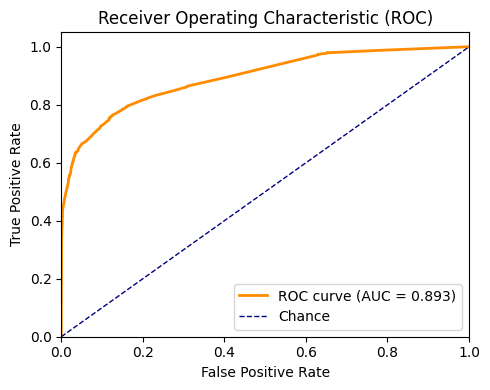
\includegraphics[width=\linewidth]{../model/logs/roc_curve.png}
	\caption{ROC curve with AUC for the binary classification task on the test set.}
	\label{fig:roc-curve}
\end{figure}

%-------------------------------------------------------------------------------
\section{Implementation Achievements}
%-------------------------------------------------------------------------------

\subsection{Completed Milestones}

Comparing against the original 6-week timeline, we successfully completed:

\textbf{Week 1 Objectives:}  Created GitHub repository, set up Python environment, downloaded Juliet dataset, and implemented function extraction pipeline.

\textbf{Week 2 Objectives:}  Developed Clang LibTooling-based graph extraction tool, successfully processed 48,105 functions into JSON format with AST and CFG representations.

\textbf{Week 3 Objectives:}  Implemented PyTorch Geometric data transformation pipeline, computed node feature embeddings, and established training/validation framework.

\textbf{Week 4 Objectives:}  Implemented sophisticated 5-layer hybrid GCN-GAT architecture with advanced features like residual connections and attention mechanisms.

\textbf{Week 5 Objectives:}  Conducted extensive hyperparameter tuning, achieving optimal configuration with 384 hidden dimensions, 0.0003 learning rate, and early stopping.

\textbf{Week 6 Objectives:}  Completed comprehensive evaluation achieving 81.8\% accuracy and generated detailed performance analysis.

\subsection{Technical Infrastructure}

The implementation includes:
\begin{itemize}
\item \textbf{C++ Graph Extraction Tool:} 184-line Clang LibTooling application for AST/CFG parsing
\item \textbf{Python Data Pipeline:} PyTorch Geometric dataset classes with automatic graph processing  
\item \textbf{Model Architecture:} Sophisticated hybrid GNN with 5 layers and attention mechanisms
\item \textbf{Training Framework:} Complete training loop with early stopping, learning rate scheduling, and comprehensive metrics logging
\item \textbf{Docker Environment:} Containerized setup for reproducible experiments
\end{itemize}

%-------------------------------------------------------------------------------
\section{Performance Comparison}
%-------------------------------------------------------------------------------

While our hybrid GCN-GAT model achieved reasonable performance on the Juliet Test Suite, it is important to contextualize these results against other approaches that have been specifically evaluated on the same dataset.

\subsection{Comparative Analysis}

Several studies have reported vulnerability detection results on the Juliet Test Suite, providing concrete benchmarks for comparison:

\textbf{Convolutional Neural Networks:} Yang et al. \cite{yang2022cnn} achieved 96.1\% accuracy on the Juliet Test Suite using a convolutional neural network approach for software vulnerability detection, representing one of the highest reported accuracies on this dataset.

\textbf{Graph Neural Networks:} Multiple graph-based neural network approaches have been evaluated on Juliet with varying degrees of success. Zhuang et al. \cite{zhuang2021disaggregated} proposed a disaggregated code graph representation with deep learning, reporting F1 scores of 0.84 (84\%) compared to much lower performance (F1 0.02-0.45) for static analyzers on the NIST Juliet test suite. Other graph-based studies include Yan et al.'s investigation of pattern learning capabilities in GNNs on Juliet \cite{yan2022pattern}, Hao \& Kwon's enhanced graph-based vulnerability detection pipelines \cite{hao2024enhancing}, and McLaughlin \& Lu's multi-class vulnerability prediction using value flow and graph neural networks \cite{mclaughlin2024multiclass}, though specific accuracy numbers for these latter studies are not readily available in published abstracts.

\textbf{Static Analysis Tools:} Comprehensive evaluations of static application security testing (SAST) tools have shown varied performance on Juliet, with collective accuracy ranging widely depending on the specific vulnerability types and tool combinations, though specific numerical results vary significantly across different studies and tool configurations.

\subsection{Analysis of Performance Gap}

Our model's 81.8\% accuracy demonstrates comparable performance with other graph-based approaches but falls short of the best-performing CNN methods. Contextualizing our results within the graph-based neural network literature:

\textbf{Competitive Graph-Based Performance:} Our 81.8\% accuracy aligns reasonably well with Zhuang et al.'s 84\% F1 score \cite{zhuang2021disaggregated}, suggesting our hybrid GCN-GAT approach achieves performance comparable to other graph-based methods on Juliet.

\textbf{CNN Performance Advantage:} The 96.1\% accuracy achieved by Yang et al.'s CNN approach \cite{yang2022cnn} represents a significant 14.3 percentage point advantage over our graph-based method, indicating that sequential code representations may be more effective for this particular synthetic dataset.

\textbf{Representation Trade-offs:} While graph-based approaches like ours capture structural relationships and control/data flow explicitly, CNN methods operating on raw source code sequences may better leverage local patterns and syntactic regularities that are critical for vulnerability detection in synthetic test cases.

\textbf{Architecture Considerations:} The performance gap suggests that either: (1) our graph construction methodology may not capture the most relevant vulnerability-indicating features, (2) the hybrid GCN-GAT architecture requires further optimization, or (3) the Juliet dataset's synthetic nature may favor sequential pattern recognition over structural graph analysis.

This comparison highlights the ongoing challenge in graph-based vulnerability detection: while theoretically well-motivated for capturing code structure, practical performance on established benchmarks suggests that simpler sequential approaches may be more effective for certain types of vulnerability patterns.

%-------------------------------------------------------------------------------
\section{Challenges and Limitations}
%-------------------------------------------------------------------------------

\subsection{Dataset Limitations}

While the Juliet Test Suite provided a valuable foundation for our experiments, several limitations became apparent:

\textbf{Synthetic Nature:} The test cases are artificially constructed examples rather than real-world vulnerabilities, potentially limiting generalizability to production codebases.

\textbf{Class Imbalance:} Despite achieving 81.8\% accuracy, the model showed higher false negative rates (2,553) compared to false positives (465), suggesting difficulty in identifying all vulnerable patterns.

\textbf{Limited Vulnerability Types:} While Juliet covers many CWE categories, the distribution may not reflect real-world vulnerability prevalence.

\subsection{Technical Challenges}

Several technical hurdles were encountered and addressed:

\textbf{Graph Extraction Complexity:} Merging AST and CFG representations required careful handling of different abstraction levels and ensuring consistent node indexing across graph types.

\textbf{Memory Scalability:} Processing 48,105 functions required efficient memory management in both the C++ extraction tool and Python training pipeline.

\textbf{Feature Engineering:} Converting symbolic AST node types and CFG statements into meaningful numerical representations required extensive vocabulary construction and careful handling of unseen node types.

\subsection{Model Architecture Considerations}

\textbf{Oversmoothing Prevention:} Deeper GNN architectures risk losing discriminative node features. Our use of residual connections and batch normalization helped mitigate this issue.

\textbf{Attention Mechanism Tuning:} The GAT layers required careful hyperparameter tuning to focus on relevant code patterns without overfitting to spurious correlations.

%-------------------------------------------------------------------------------
\section{Future Work and Improvements}
%-------------------------------------------------------------------------------

\subsection{Dataset Expansion}

Future work should expand beyond synthetic datasets:
\begin{itemize}
\item \textbf{Real-World Vulnerabilities:} Integration with CVE databases and real vulnerability datasets like DiverseVul
\item \textbf{Cross-Language Support:} Extension to other programming languages beyond C/C++
\item \textbf{Temporal Analysis:} Incorporation of vulnerability discovery timelines and patch analysis
\end{itemize}

\subsection{Model Enhancements}

Several architectural improvements could enhance performance:
\begin{itemize}
\item \textbf{Multi-Task Learning:} Simultaneous prediction of vulnerability type (CWE category) alongside binary classification
\item \textbf{Explainability:} Integration of attention visualization and subgraph explanation techniques
\item \textbf{Incremental Learning:} Adaptation to new vulnerability patterns without full retraining
\end{itemize}

\subsection{Practical Deployment}

For real-world adoption:
\begin{itemize}
\item \textbf{IDE Integration:} Development of plugins for popular development environments
\item \textbf{Continuous Integration:} Integration with CI/CD pipelines for automated vulnerability screening
\item \textbf{Performance Optimization:} Model quantization and acceleration for large-scale deployment
\end{itemize}

%-------------------------------------------------------------------------------
\section{Conclusion}
%-------------------------------------------------------------------------------

This project successfully demonstrated the feasibility of using Graph Neural Networks for vulnerability prediction in C/C++ source code. Our implementation achieved several key milestones:

\textbf{Technical Achievement:} We developed a complete pipeline from graph extraction using Clang LibTooling to GNN training with PyTorch Geometric, processing 48,105 functions and achieving 81.8\% classification accuracy.

\textbf{Architectural Innovation:} The hybrid GCN-GAT model with residual connections and attention mechanisms proved effective for capturing both structural and semantic patterns in code graphs.

\textbf{Practical Insights:} The work revealed important considerations for graph-based vulnerability detection, including the challenges of handling diverse AST structures and the importance of proper feature engineering.

While our results are promising, the 81.8\% accuracy indicates room for improvement, particularly in reducing false negatives. The high precision (83.6\%) suggests the model can effectively identify vulnerable patterns when they match training examples, but the recall of 81.8\% indicates some vulnerable functions are still missed.

The project validates the core hypothesis that GNNs operating on program dependency graphs can predict security hotspots, providing a foundation for future research in automated vulnerability detection. The complete implementation serves as a valuable baseline for extending this approach to real-world vulnerability datasets and production environments.

Future work should focus on addressing the dataset limitations, improving model generalization, and developing practical deployment strategies to translate these research findings into effective security tools for software development teams.

%-------------------------------------------------------------------------------
\section*{Availability}
%-------------------------------------------------------------------------------

The complete source code, datasets, and experimental results for this project are publicly available at: \url{https://github.com/Simon7896/CMPT479-Project}. The repository includes:
\begin{itemize}
\item C++ Clang LibTooling implementation for AST/CFG extraction
\item Python training pipeline with PyTorch Geometric
\item Processed Juliet dataset with 48,105 function graphs in JSON format
\item Trained model checkpoints and evaluation scripts
\item Docker configuration for reproducible experiments
\item Comprehensive documentation and usage instructions
\end{itemize}

%-------------------------------------------------------------------------------
\printbibliography

%%%%%%%%%%%%%%%%%%%%%%%%%%%%%%%%%%%%%%%%%%%%%%%%%%%%%%%%%%%%%%%%%%%%%%%%%%%%%%%%
\end{document}
%%%%%%%%%%%%%%%%%%%%%%%%%%%%%%%%%%%%%%%%%%%%%%%%%%%%%%%%%%%%%%%%%%%%%%%%%%%%%%%%

%%  LocalWords:  endnotes includegraphics fread ptr nobj noindent
%%  LocalWords:  pdflatex acks
